\chapter{Ethernet}

L'Ethernet è il sistema di comunicazione per computer più diffuso.\
Ha avuto un gran successo perché è un sistema molto semplice (ciò non vuol dire che fosse il migliore).\

Nella versione iniziale Ethernet è semplicemente un filo, un cavo coassiale (simile a quello della TV) alle cui estremità ci sono due resistenze, chiamate \textit{terminatori}, che impediscono effetti di disturbo (``rimbalzi di segnale'').

Le stazioni che vogliono connettersi alla rete hanno un ``vampire'' tap per collegarsi al cavo Ethernet.\
A questo tap era attacato un cavo che terminava nell'Ethernet Controller (scheda di rete) della stazione.

\begin{figure}[H]
    \centering
    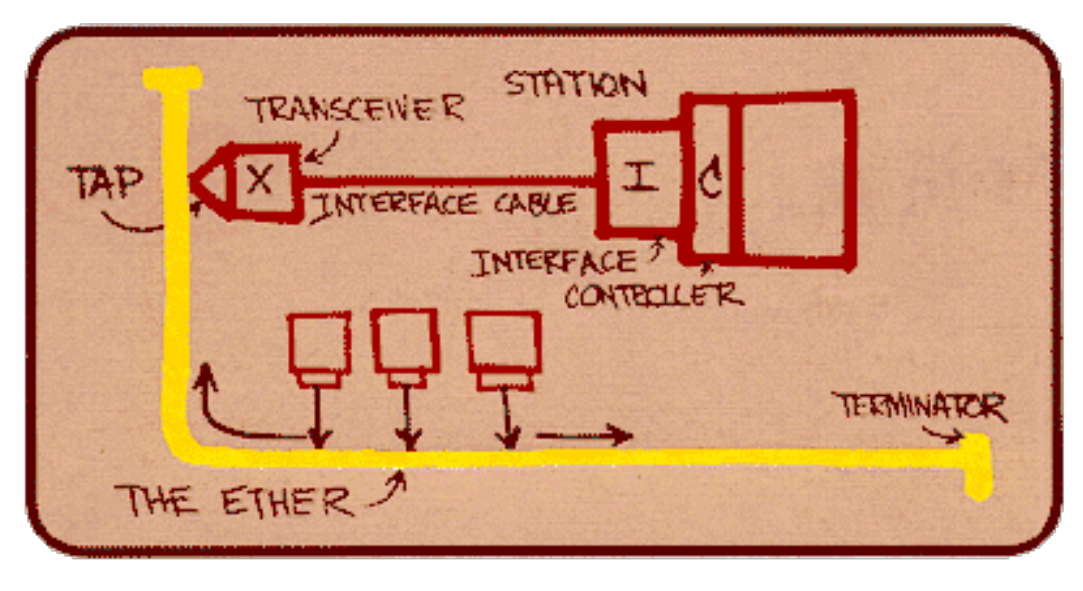
\includegraphics[width=0.4\textwidth]{immagini/Ethernet.png}
    \caption*{Bob Metcalfe, mid 1970s}
\end{figure}

\noindent Nel tempo questa tipologia è cambiata, da prima andando a utilizzare un connettore a T al posto del ``vampire'' tap.

\begin{figure}[H]
    \centering
    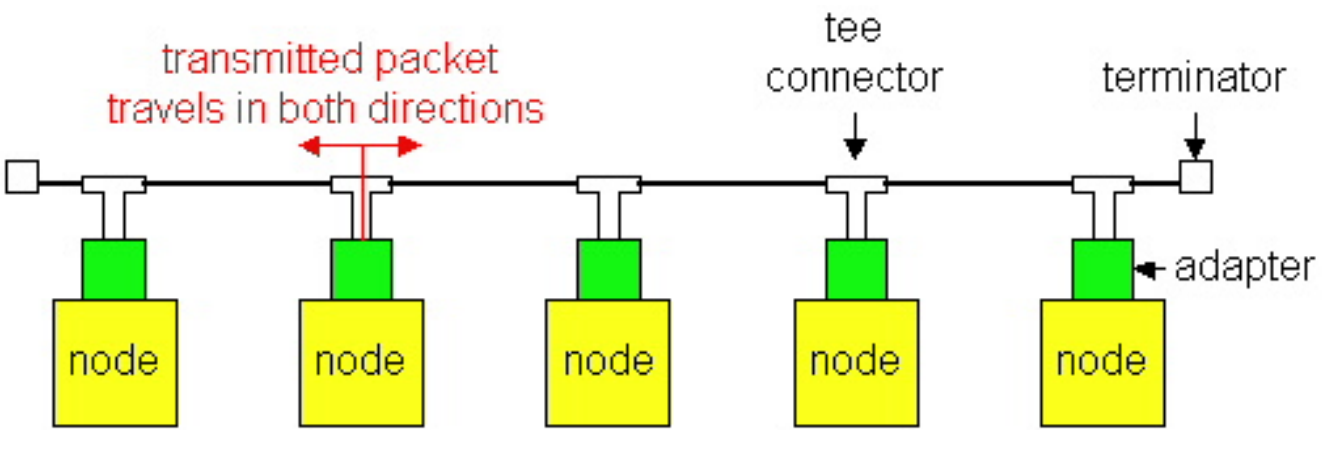
\includegraphics[width=0.4\textwidth]{immagini/Ethernet_bus.png}
    \caption*{Bus Topology\\(10Base2 - 802.3a-1988)}
\end{figure}
\noindent Negli anni `90 si è poi diffusa la tipologia a stella, in cui abbiamo uno hub/switch al quale i computer si connettono con un cavo di rete.

\begin{figure}[H]
    \centering
    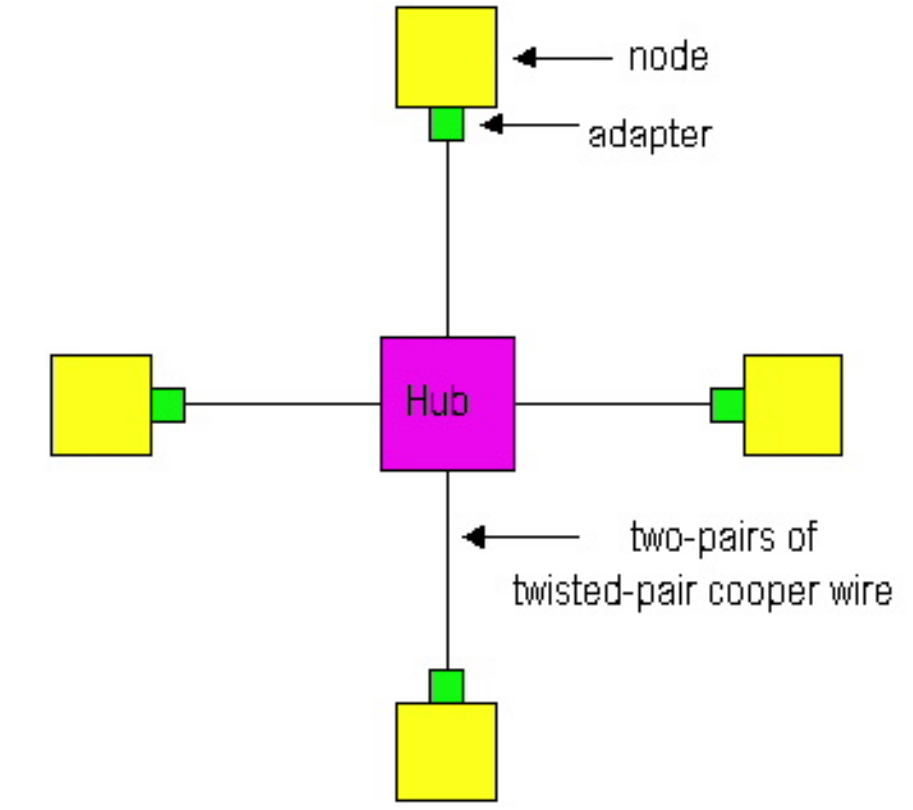
\includegraphics[width=0.4\textwidth]{immagini/Ethernet_hub.png}
    \caption*{Star topology\\ (10/100BaseT - 802.3i-1990)}
\end{figure}

\noindent La differenza principale tra le due implementazioni è che nella prima soluzione il collegamento è condiviso da tutti i nodi connessi, ciò comporta la possibilità di avere delle ``collisioni'', mentre con la struttura a stella si hanno dei collegamenti punto-punto.\

Ethernet può funzionare in \textbf{half-duplex} (storico) e \textbf{full-duplex} come specificato in 802.3x (ethernet moderno).\
In modalità full duplex, le stazioni possono trasmettere e ricevere simultaneamente poiché non vi è alcun conflitto per l'utilizzo del supporto condiviso.

\begin{figure}[H]
    \centering
    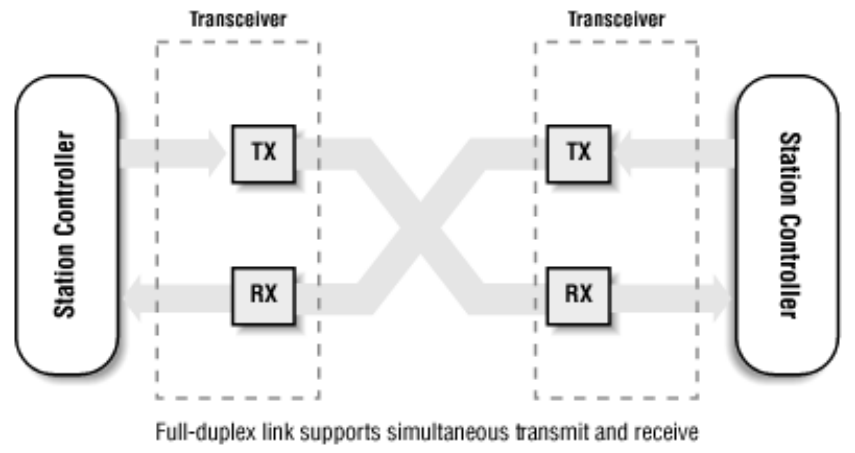
\includegraphics[width=0.5\textwidth]{immagini/FullDuplex.png}
\end{figure}

\subsubsection{PoE (Power over Ethernet)}

L'Ethernet oggi non è usato solo per trasmettere dati, ma anche per fornire alimentazione.\

Standard \textbf{PoE} (Power over Ethernet):\ soluzione elegante per unire dati e alimentazione utilizzata principalmente per dispositivi a bassa potenza come antenne e punti di accesso WiFi.\
PoE Type 2: 25.5 W, 600 mA.

\begin{figure}[H]
    \centering
    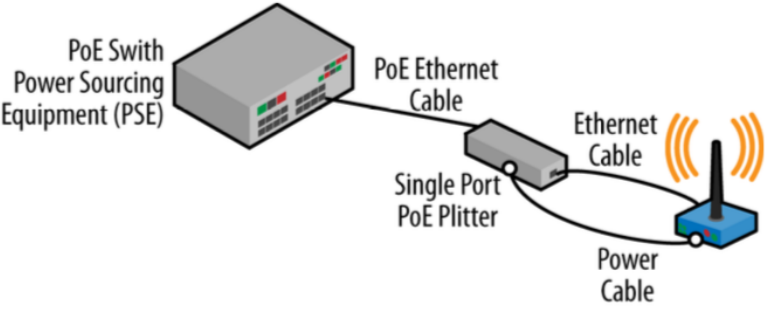
\includegraphics[width=0.5\textwidth]{immagini/PoE.png}
\end{figure}

\subsubsection{Ethernet Pinout}

La Ethernet è composta da otto cavi accoppiati come mostrato in figura.\

\begin{figure}[H]
    \centering
    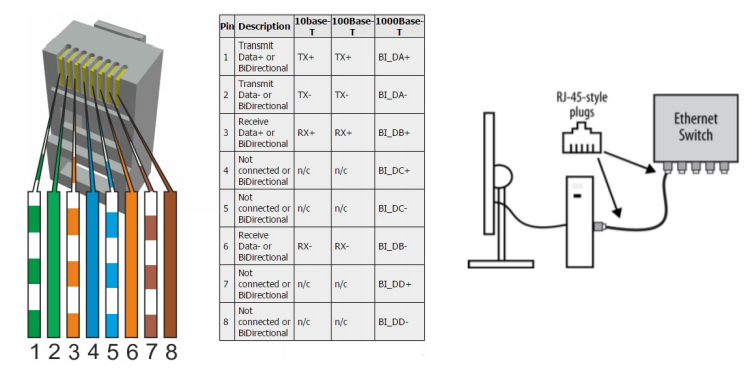
\includegraphics[width=\textwidth]{immagini/Ethernet_pinout.png}
\end{figure}

\noindent Esiste un ulteriore metodo di accompiamento in cui i cavi sono accoppiati per colore.

Alternativamente esistono i cablaggi in fibra ottica.\
Tipicamente sono composti da due fibre fisicamente separate, ma unite da un ``cappuccio'' che serve per tenerle insieme.

\begin{figure}[H]
    \centering
    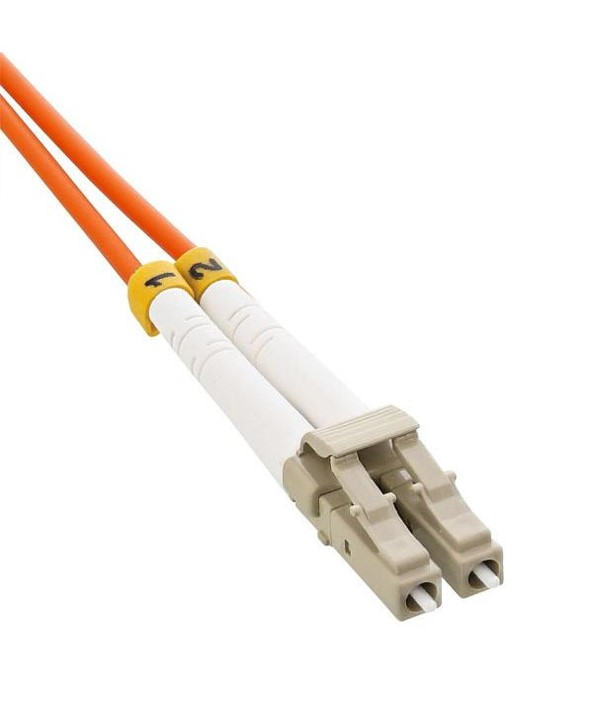
\includegraphics[width=0.2\textwidth]{immagini/FibraOttica_cavo.jpg}
    \caption*{Cavo della fibra ottica}

\end{figure}

\begin{figure}[H]
    \centering
    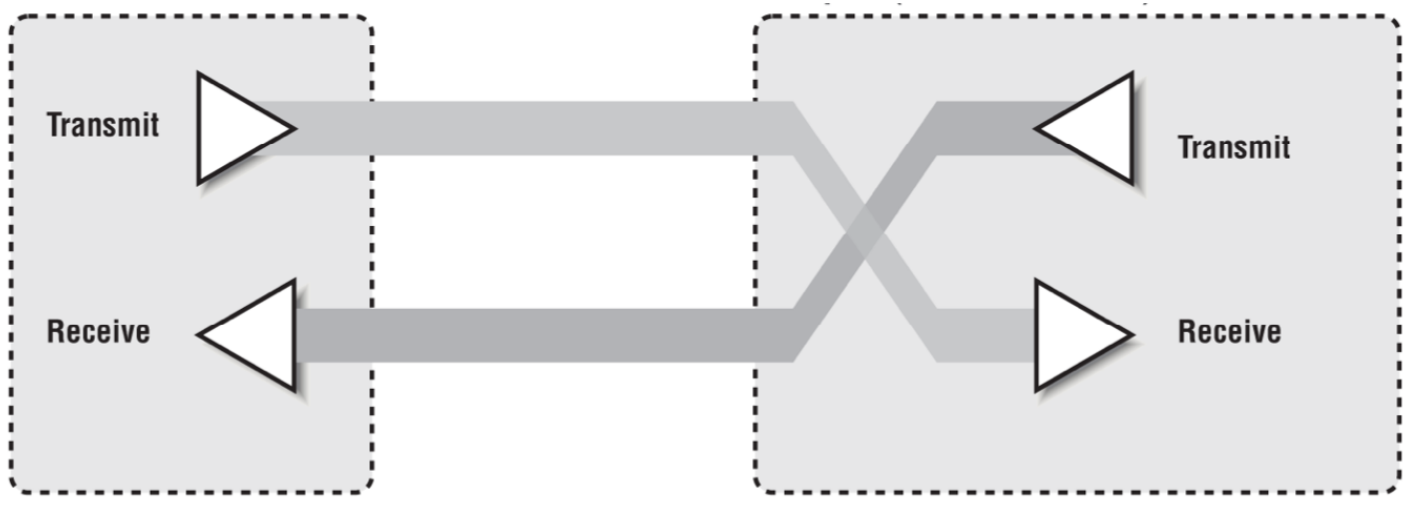
\includegraphics[width=0.8\textwidth]{immagini/FibraOttica.png}
    \caption*{Fibra ottica}
\end{figure}

\noindent Nella fibra a 40 Gbit si usano quattro cavi da 10 Gbit collegati a un ``distributore'' \textit{round-robin}.\
Nella 100 Gbit si usano dieci cavi 10 Gbit accoppiati tra loro.\
Questo perché spesso, invece di partire da zero, si parte da qualcosa di esistente e lo si adatta alle esigenze.\

\begin{figure}[H]
    \centering
    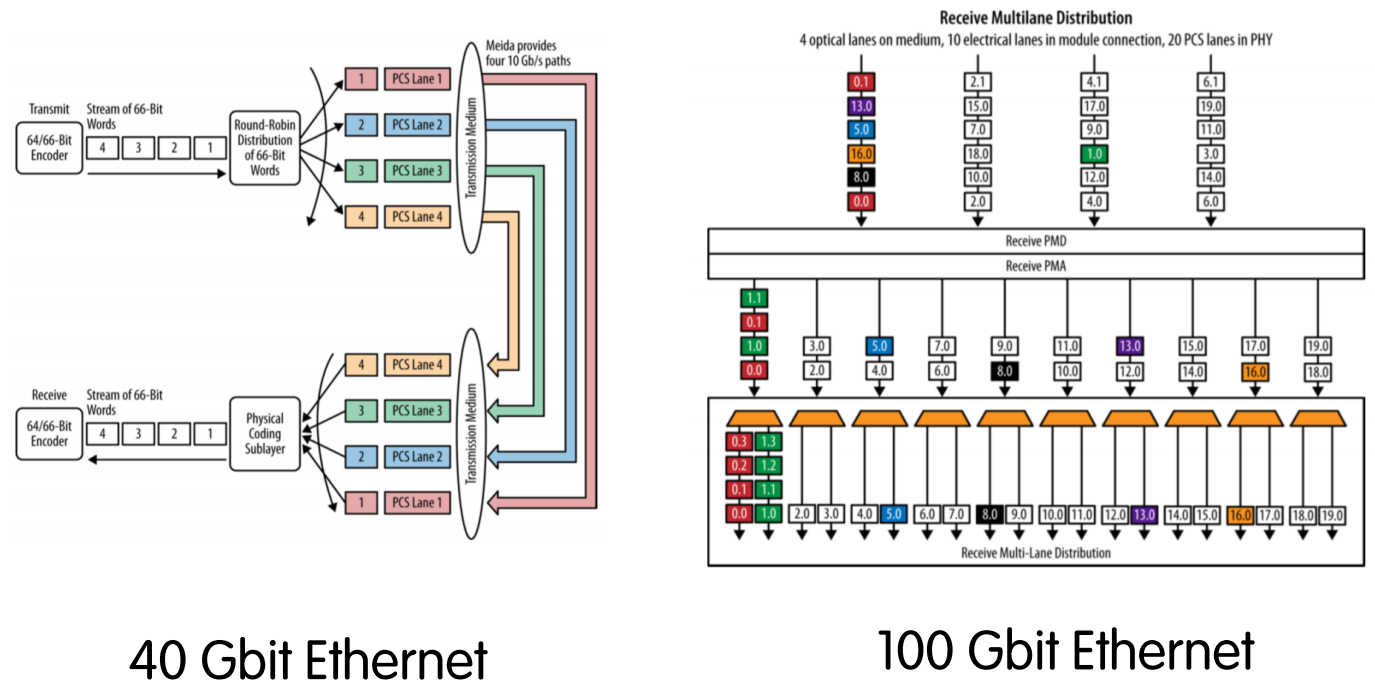
\includegraphics[width=\textwidth]{immagini/40_100_Gbit.png}
    \caption*{Primi standard}
\end{figure}

\subsubsection{Ethernet Flow Control}

Il controllo del flusso è un meccanismo utilizzato dal ricevitore (il ricevitore è il re!)\ per richiedere al mittente una breve pausa nella trasmissione del frame inviando un comando \texttt{PAUSE} all'indirizzo multicast di destinazione 01:80:C2:00:00:01.

\begin{figure}[H]
    \centering
    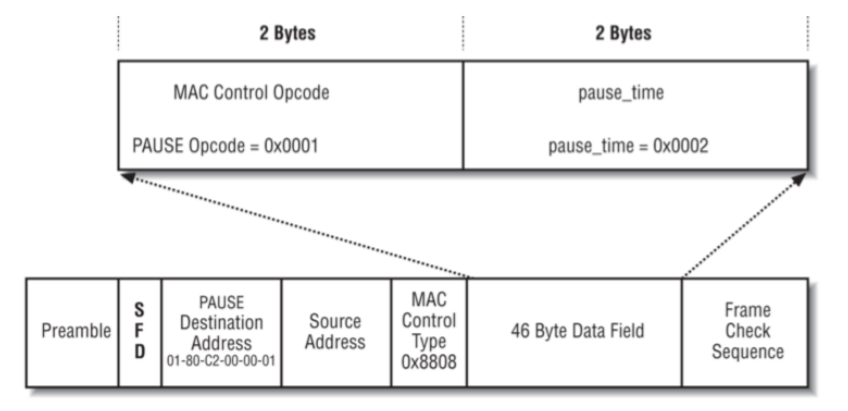
\includegraphics[width=0.6\textwidth]{immagini/Flow_control.png}
\end{figure}

\noindent In alcuni casi l'uso dei \texttt{PAUSE} frame non risulta molto comodo, come nel caso in cui si vuole testare la capacità di una scheda di rete.\
In questo caso (su Linux) si può usare il comando \texttt{ethtool} per specificare di ignorare i \texttt{PAUSE} frame.

\section{Ethernet Framing}

\begin{figure}[H]
    \centering
    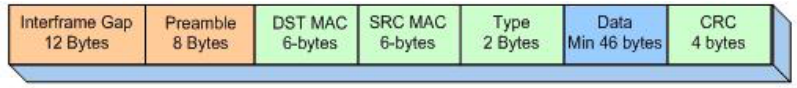
\includegraphics[width=\textwidth]{immagini/Ethernet_framing.png}
\end{figure}

\noindent \textbf{Interframe Gap}:\ pausa (tempo) minima tra i pacchetti che consente al ricevitore di prepararsi per il frame successivo (96 nsec su Gbit Ethernet).

\noindent\textbf{Preamble}:\ una sequenza di 56 bit 0/1 alternati seguita da 8 bit a 1, consentendo al mittente di sincronizzarsi con il ricevitore.

\noindent\textbf{CRC}:\ sequenza di controllo del frame basata sull'utilizzo del CRC (Cyclic Redundancy Check) per rilevare (ma non correggere) gli errori di trasmissione.

Questi meccanismi permettono l'assenza del campo che indica la lunghezza dei dati trasmessi.

La dimensione minima del pacchetto Ethernet è di 60 byte:\ i frame più corti sono riempiti.

\begin{table}[H]
    \centering
    \begin{tabular}{|l|l|}
        \hline
        IFG                    & 12          \\\hline
        Preamble               & 8           \\\hline
        Min Ethernet Frame     & 60          \\\hline
        CRC                    & 4           \\\hline
        \hline
        \textbf{Total (bytes)} & \textbf{84} \\\hline
    \end{tabular}
\end{table}

\begin{figure}[H]
    \centering
    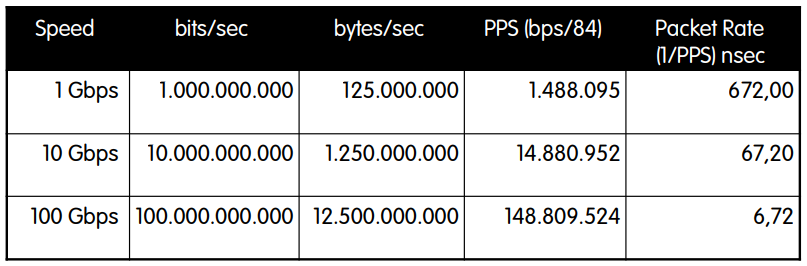
\includegraphics[width=0.7\textwidth]{immagini/Ethernet_speed.png}
\end{figure}

\section{Operation of Ethernet Switches}

Gli switch Ethernet sono dispositivi ``invisibili'' alla rete, in quanto non modificano i frame Ethernet collegati a ponte tra le porte, e non richiedono alcuna configurazione poiché apprendono la topologia e la configurazione della rete analizzando il traffico di rete.

\begin{figure}[H]
    \centering
    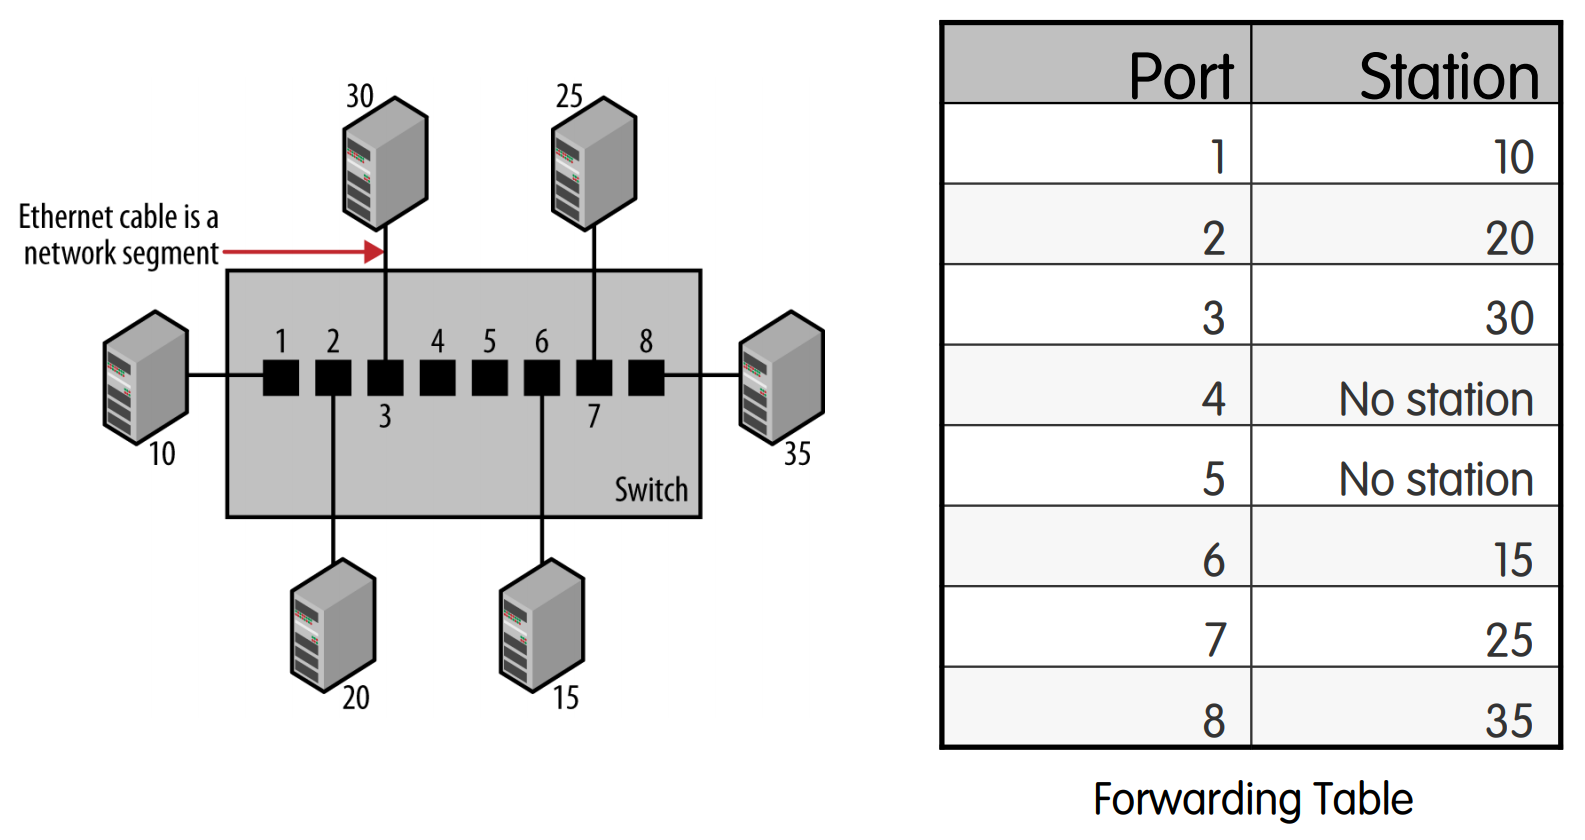
\includegraphics[width=0.6\textwidth]{immagini/Switch.png}
\end{figure}

\noindent Le stazioni pubblicizzano la loro presenza inviando frame ethernet; la tabella di inoltro viene riempita dinamicamente e automaticamente (nessuna configurazione) man mano che vengono ricevuti i pacchetti in entrata.\
Poiché lo switch può essere annidato in un'architettura ad albero{\slash}mesh, è possibile collegare più stazioni alla stessa porta.

Il traffico viene inoltrato in base all'indirizzo ethernet di destinazione:

\begin{itemize}
    \item Quando viene ricevuto un frame, il MAC di destinazione viene cercato nella tabella di inoltro.
    \item Se trovato, i frame vengono inviati alla stazione di destinazione (layer 2 anycast).
    \item Altrimenti il traffico viene inviato a tutte le porte tranne quella da cui è stato ricevuto il frame (broadcast layer 3).
\end{itemize}

\noindent\textbf{Nota bene}:\ le \textbf{VLAN} influiscono sull'inoltro del traffico creando più domini di broadcast.\
Al campo \texttt{Type} dell'Ethernet frame viene aggiunto un tag che identifica un dominio:\ i pacchetti mandati in broadcast su una VLAN non vengono trasmessi all'esterno di essa.

\begin{figure}[H]
    \centering
    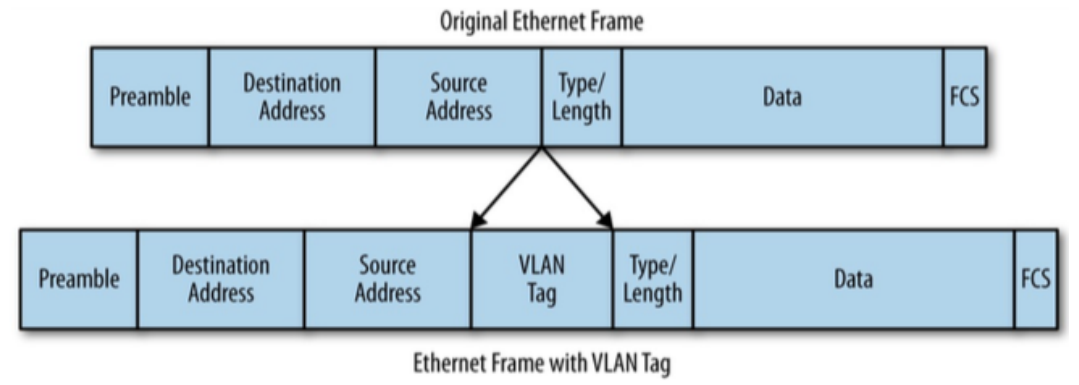
\includegraphics[width=0.7\textwidth]{immagini/VLAN_tag.png}
    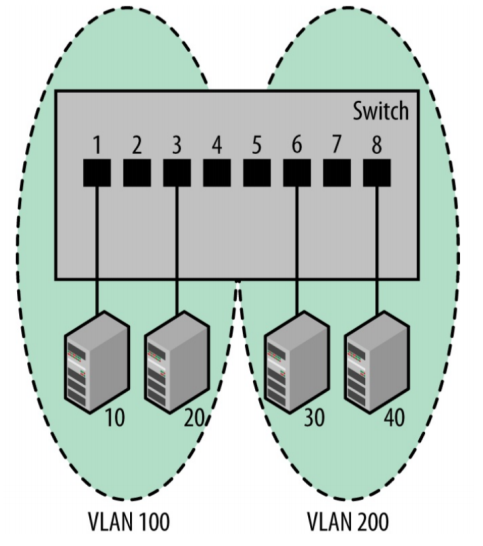
\includegraphics[width=0.3\textwidth]{immagini/VLAN_domain.png}
\end{figure}

\noindent Poiché Ethernet richiede che esista un solo percorso tra due stazioni qualsiasi, esistono dei protocolli che permettono a degli switch di disabilitare alcuni link (sempre attivi dal punto di vista elettrico) nel caso in cui ``capiscano'' che esiste un loop.

\begin{figure}[H]
    \centering
    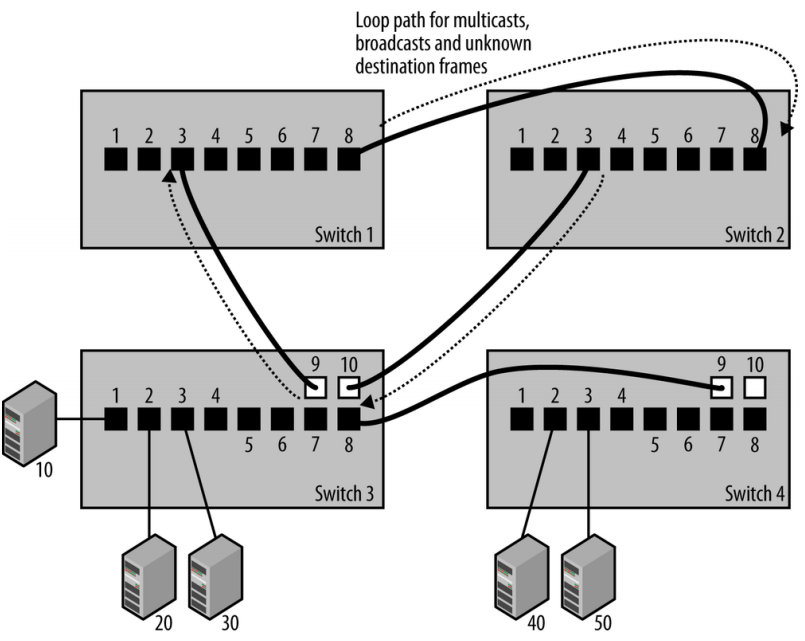
\includegraphics[width=0.7\textwidth]{immagini/Loop_path.png}
\end{figure}
